\documentclass[11pt,a4paper]{article}

\usepackage[margin=2.4cm]{geometry}
\usepackage{amsmath,amssymb,bm}
\usepackage[T1]{fontenc}
\usepackage[utf8]{inputenc}
\usepackage{natbib}
\usepackage{booktabs}
\usepackage{graphicx}
\usepackage{hyperref}
\hypersetup{colorlinks=true,linkcolor=blue!50!black,citecolor=blue!50!black,urlcolor=blue!50!black}
\usepackage{xcolor}

\bibliographystyle{plainnat}
\setcitestyle{authoryear,round}

\newcommand{\Ndot}{\dot{N}_{\rm ion}}
\newcommand{\aB}{\alpha_{\rm B}}
\newcommand{\nH}{n_{\rm H}}
\newcommand{\HII}{\ion{H}{ii}}
\newcommand{\ion}[2]{\textrm{#1\,\textsc{#2}}}
\newcommand{\pMpc}{\,{\rm pMpc}}
\newcommand{\cMpc}{\,{\rm cMpc}}
\newcommand{\Msun}{\,M_\odot}

\title{\bf How Does Reionization Complete If Individual\\ Star-Forming-Galaxy Bubbles Stay Below $1$~Mpc?\\[2mm]
\large Response record for \texttt{reionization\_completion.py}, following Master Rule 2}
\author{Prepared for L.\ Carvalho}
\date{4 September 2026}

\begin{document}
\maketitle

\begin{abstract}
\noindent
\texttt{bubble\_radius\_vs\_redshift.png} and \texttt{bubble\_radius\_vs\_redshift\_planckXHI.png} show that
the ionized bubble of one fiducial star-forming galaxy ($\mathrm{SFR}=10\Msun\,{\rm yr^{-1}}$) never exceeds
$\sim1\pMpc$ for $6\le z\le18$. This is not a contradiction with cosmic reionization being complete by
$z\sim5$--$8$: reionization is not the growth of a single bubble to cosmological size, but the
\emph{collective overlap} of the bubbles of the entire, numerous, star-forming-galaxy population. This note
makes that resolution quantitative using two independent, cross-checked calculations
(Sec.~\ref{sec:derivation}), both built entirely from ingredients already cited in this folder: the global
ionized-volume-filling-factor equation of \citet{Choudhury2022} driven by the cosmic star-formation-rate
density of \citet{MadauDickinson2014}, and a percolation argument comparing the single-galaxy bubble radius
to the mean separation between galaxies implied by that same star-formation-rate density. It documents
\texttt{reionization\_completion.py} (same folder), which produced \texttt{reionization\_completion.png}.
\end{abstract}

\tableofcontents

%=====================================================================
\section{Assumptions}
\label{sec:assumptions}

\begin{enumerate}
\item The single-galaxy bubbles of \texttt{bubble\_radius\_response.tex} represent the ionized volume
      produced by \emph{one} galaxy's own photon budget. Explaining global reionization requires instead the
      \emph{ionized volume filling factor} $Q_{\rm HII}(z)$, the standard quantity used throughout the
      reionization literature (e.g.\ \citealt{Choudhury2022}, already in \texttt{references/}, their eq.~66,
      reproduced as eq.~\texttt{QHII} of \texttt{stromgren\_sphere\_summary.tex}).
\item $Q_{\rm HII}(z)$ is driven by the ionizing photon output of the \emph{entire} star-forming-galaxy
      population, encoded through the cosmic star-formation-rate density $\rho_{\rm SFR}(z)$ of
      \citet{MadauDickinson2014} (already in \texttt{references/}), \emph{not} by one representative galaxy.
      The same $\xi_{\rm ion}(z)$ \citep{Llerena2024}, $f_{\rm esc}=0.2$ \citep{Robertson2015}, and
      $\kappa_{\rm FUV}$ \citep{MadauDickinson2014} used for the single-galaxy calculation are reused here,
      for direct comparability.
\item Recombinations use $\alpha_B(10^4\,{\rm K})=2.59\times10^{-13}\,{\rm cm^3\,s^{-1}}$ (already established
      in \texttt{check\_consistency.py}, \citealt{Shapiro2006}) and a clumping factor $C_{\rm HII}=3$
      \citep{Robertson2015}, with a sensitivity band down to $C=1$; using $\alpha_B$ at $10^4$~K rather than
      the $2\times10^4$~K adopted alongside $C=3$ by \citet{Robertson2015} is an explicit, flagged
      approximation (see Sec.~\ref{sec:verification}).
\item Cosmology and formation redshift are identical to the previous two tasks: Planck 2018
      \citep{Planck2018VI}, $z_{\rm form}=20$ \citep{Kitayama2004}.
\item The percolation argument treats the cosmic SFRD as if it were produced entirely by galaxies
      equivalent to the fiducial $\mathrm{SFR}=10\Msun\,{\rm yr^{-1}}$ source used in the bubble-radius
      calculation, purely to estimate a characteristic comoving number density and mean separation --- an
      explicit simplification of the true, extended luminosity function, stated here rather than hidden.
\end{enumerate}

%=====================================================================
\section{Derivation}
\label{sec:derivation}

\subsection{(A) The global ionized-volume-filling-factor equation}
Following \citet{Choudhury2022} (their eq.~66; eq.~\texttt{QHII} of \texttt{stromgren\_sphere\_summary.tex}):
\begin{equation}
  \frac{\mathrm{d}Q_{\rm HII}}{\mathrm{d}t} \;=\; \frac{\dot n_\gamma(z)}{n_{{\rm H},0}}
  \;-\; Q_{\rm HII}\,a^{-3}\,C\,\alpha_B(T)\,\bar n_e(z),
  \label{eq:QHII}
\end{equation}
with the ionizing emissivity driven by the \emph{entire} population via the cosmic SFRD,
\begin{equation}
  \dot n_\gamma(z) \;=\; f_{\rm esc}\,\xi_{\rm ion}(z)\,\frac{\rho_{\rm SFR}(z)}{\kappa_{\rm FUV}}, \qquad
  \rho_{\rm SFR}(z) = \frac{0.015\,(1+z)^{2.7}}{1+[(1+z)/2.9]^{5.6}}\ \Msun\,{\rm yr^{-1}\,cMpc^{-3}}
  \label{eq:rhoSFR}
\end{equation}
\citep{MadauDickinson2014}, and $\bar n_e(z)=\chi_{\rm He}\,n_{{\rm H},0}(1+z)^3$, $\chi_{\rm He}=1.08$.
\textbf{Note the crucial distinction between the two terms}: the source term uses the \emph{fixed comoving}
mean hydrogen density $n_{{\rm H},0}$ (evaluated at $z=0$), because $\dot n_\gamma$ and $Q_{\rm HII}$ are
comoving quantities, whereas the sink term carries the explicit $a^{-3}=(1+z)^3$ scale-factor dependence of
the physical recombination rate. Eq.~(\ref{eq:QHII}) is integrated numerically from $z=25$ ($Q_{\rm HII}=0$)
to $z=4$.

\subsection{(B) The percolation / bubble-overlap argument}
The comoving number density of $\mathrm{SFR}=10\Msun\,{\rm yr^{-1}}$-equivalent galaxies implied by the same
$\rho_{\rm SFR}(z)$ is
\begin{equation}
  n_{\rm gal}(z) = \frac{\rho_{\rm SFR}(z)}{\mathrm{SFR}_{\rm fid}}, \qquad
  d_{\rm sep}(z) = n_{\rm gal}(z)^{-1/3},
  \label{eq:sep}
\end{equation}
compared directly to the single-galaxy bubble radius $R_{\rm bubble}(z)$ of
\texttt{bubble\_radius\_vs\_redshift.py} (eq.~\texttt{photon\_counting}). If $d_{\rm sep}(z)\lesssim
2\,R_{\rm bubble}(z)$, neighboring bubbles are expected to touch/overlap --- the mechanism invoked
qualitatively by the excursion-set bubble-growth model of \citet{Furlanetto2004} (self-ionization condition
$f_{\rm coll}\ge\zeta^{-1}$, already eq.~\texttt{barrier} of \texttt{stromgren\_sphere\_summary.tex}) and seen
directly in radiation-hydrodynamic simulations by \citet{Neyer2023} (THESAN), who describe newly-ionized
regions undergoing ``flash ionization'' as they suddenly join a much larger, pre-existing bubble.

%=====================================================================
\section{Verification / cross-check}
\label{sec:verification}

All checks below are reproduced verbatim by running \texttt{reionization\_completion.py}.

\begin{enumerate}
\item \textbf{Sympy check.} The constant-coefficient limit of eq.~(\ref{eq:QHII}),
      $Q(t)=\tfrac{\dot n_\gamma}{n_{{\rm H},0}Ca_Bn_e}(1-e^{-Ca_Bn_et})$, is confirmed by sympy to solve
      $\mathrm{d}Q/\mathrm{d}t=\dot n_\gamma/n_{{\rm H},0}-QCa_Bn_e$ exactly (residual $=0$) --- structurally
      the same ``recombination clock'' already verified for $R(t)$ in \texttt{check\_consistency.py}.
\item \textbf{An error caught by cross-checking against a basic benchmark (Master Rule 5, in practice).} A
      first attempt at integrating eq.~(\ref{eq:QHII}) mistakenly used the \emph{physical}, diluting
      $n_{\rm H}(z)=n_{{\rm H},0}(1+z)^3$ in the source-term denominator instead of the fixed comoving
      $n_{{\rm H},0}$. This suppressed $Q_{\rm HII}$ by a factor $(1+z)^3\sim700$ at $z=8$ and predicted that
      reionization could not complete within a Hubble time at any redshift shown here --- directly
      contradicting the well-established fact that it does, by $z\sim6$ (Gunn--Peterson troughs,
      \citealt{White2003}, already in \texttt{references/}). Re-examining eq.~(\ref{eq:QHII}) as written by
      \citet{Choudhury2022} (their explicit $a^{-3}$ factor \emph{only} on the recombination term) identified
      the bug; correcting it is what produced the results below. This is reported explicitly, per Master Rule
      5, rather than silently fixed and hidden.
\item \textbf{Completion redshift vs.\ known benchmarks.} With $C=3$: $Q_{\rm HII}(z{=}9)=0.173$,
      $Q_{\rm HII}(z{=}8)=0.256$, $Q_{\rm HII}(z{=}7)=0.401$, $Q_{\rm HII}(z{=}6)=0.674$; the model reaches
      $Q_{\rm HII}=0.5$ at $z=6.56$ and $Q_{\rm HII}\simeq1$ by $z\simeq5.3$. This is broadly consistent with
      cosmic reionization completing at $z\sim5$--$6$ \citep{White2003}, though --- exactly as already flagged
      in \texttt{bubble\_radius\_response.tex} --- it is \emph{later} than the Planck 2018 CMB-only
      instantaneous-reionization estimate $z_{\rm re}=7.68\pm0.79$ \citep{Planck2018VI}: the same early/late
      reionization-history tension recurs here, now derived independently from the galaxy side rather than
      assumed.
\item \textbf{Direct cross-check against \citet{Umeda2023}.} At $z=7.12$: $1-Q_{\rm HII}({\rm model})=0.621$
      vs.\ $x_{\rm HI,\,measured}=0.53$. At $z=9.91$: $1-Q_{\rm HII}({\rm model})=0.874$ vs.\
      $x_{\rm HI,\,measured}=0.92$. Both agree to $\lesssim0.1$ in $x_{\rm HI}$ --- a non-trivial success,
      since nothing in eq.~(\ref{eq:QHII}) was tuned to match these particular measurements (unlike the
      single-galaxy $x_{\rm HI}(z)$ of \texttt{bubble\_radius\_vs\_redshift.py}, which \emph{was} fit to them).
\item \textbf{Sensitivity to the clumping factor.} Lowering $C$ from $3$ to $1$ moves $z(Q_{\rm HII}=0.5)$
      from $6.56$ to $7.50$, i.e.\ a less clumpy IGM reionizes earlier for the same photon budget, as
      expected from the sink term of eq.~(\ref{eq:QHII}).
\item \textbf{Percolation check.} At $z=8$: $R_{\rm bubble}=0.752\pMpc$ vs.\ half the mean separation
      $d_{\rm sep}/2=0.557\pMpc$ (ratio $0.74$); at $z=12$: ratio $1.33$ (bubbles not yet touching); at
      $z=6$: ratio $0.42$ (bubbles well past first contact). The two curves cross near $z\approx9.5$,
      meaning: by the time individual bubbles are only $\sim0.5$--$0.6\pMpc$ across, they are already, on
      average, as close to their nearest neighbor as their own radius --- overlap is generic from
      $z\lesssim9$--10 onward, well before any single bubble needs to grow beyond $\sim1\pMpc$.
\item \textbf{Independent, cruder cross-check: naive non-overlapping packing.} Defining
      $Q_{\rm naive}(z)\equiv n_{\rm gal}(z)\,\tfrac{4}{3}\pi\,[R_{\rm bubble}(z)(1+z)]^3$ (comoving volume of
      non-overlapping spheres, ignoring recombinations and overlap): $Q_{\rm naive}(z{=}8)=1.29$,
      $Q_{\rm naive}(z{=}7)=2.74$, $Q_{\rm naive}(z{=}6)=6.95$ --- \emph{exceeding unity} already at
      $z\lesssim8$. A packing fraction $>1$ for non-overlapping spheres is unphysical by construction, so
      this is itself direct, independent evidence that the bubbles \emph{must} already be overlapping
      substantially at these redshifts; the self-consistent $Q_{\rm HII}$ from eq.~(\ref{eq:QHII}) (item 3),
      which properly subtracts recombination losses, is correspondingly and expectedly lower.
\end{enumerate}

%=====================================================================
\section{Final result}
\label{sec:final}

Reionization completes not because any single star-forming galaxy's bubble grows to a cosmologically large
size, but because (i) the mean separation between star-forming galaxies shrinks with cosmic time faster than
any individual bubble needs to grow, so neighboring bubbles start overlapping already around
$z\approx9$--$10$ (Sec.~\ref{sec:verification}, item~6); and (ii) the \emph{cumulative} ionizing output of
the entire population --- not of one galaxy --- is what the global filling factor $Q_{\rm HII}(z)$ tracks,
reaching $Q_{\rm HII}=0.5$ at $z=6.56$ and $Q_{\rm HII}\simeq1$ by $z\simeq5.3$ for the fiducial parameters
adopted here (Sec.~\ref{sec:verification}, item~3), consistent with $x_{\rm HI}(z)$ measured directly by
\citet{Umeda2023} to within $\lesssim0.1$ (item~4) and, order-of-magnitude, with the Gunn--Peterson
constraint that reionization is essentially complete by $z\sim6$ \citep{White2003}. This is exactly the
``inside-out, then overlap'' qualitative picture already described in
\texttt{stromgren\_sphere\_summary.tex} (\citealt{Chakraborty2025,Cen2000}: \emph{``isolated ionized bubbles
form around the first sources, then grow, overlap and finally fill the IGM, leaving neutral gas only in
dense pockets''}) and in the excursion-set bubble-size-distribution formalism of \citet{Furlanetto2004},
made quantitative here for the specific fiducial galaxy of the previous two tasks. The dominant explicitly
quoted systematic is the clumping factor ($C=1$ vs.\ $3$ shifts $z(Q_{\rm HII}=0.5)$ from $7.50$ to $6.56$,
item~5), and the calculation reproduces --- rather than resolves --- the already-known tension between the
Planck CMB-only $z_{\rm re}=7.68$ and the later completion redshift implied by direct galaxy/IGM probes.

\begin{figure}[h]
\centering
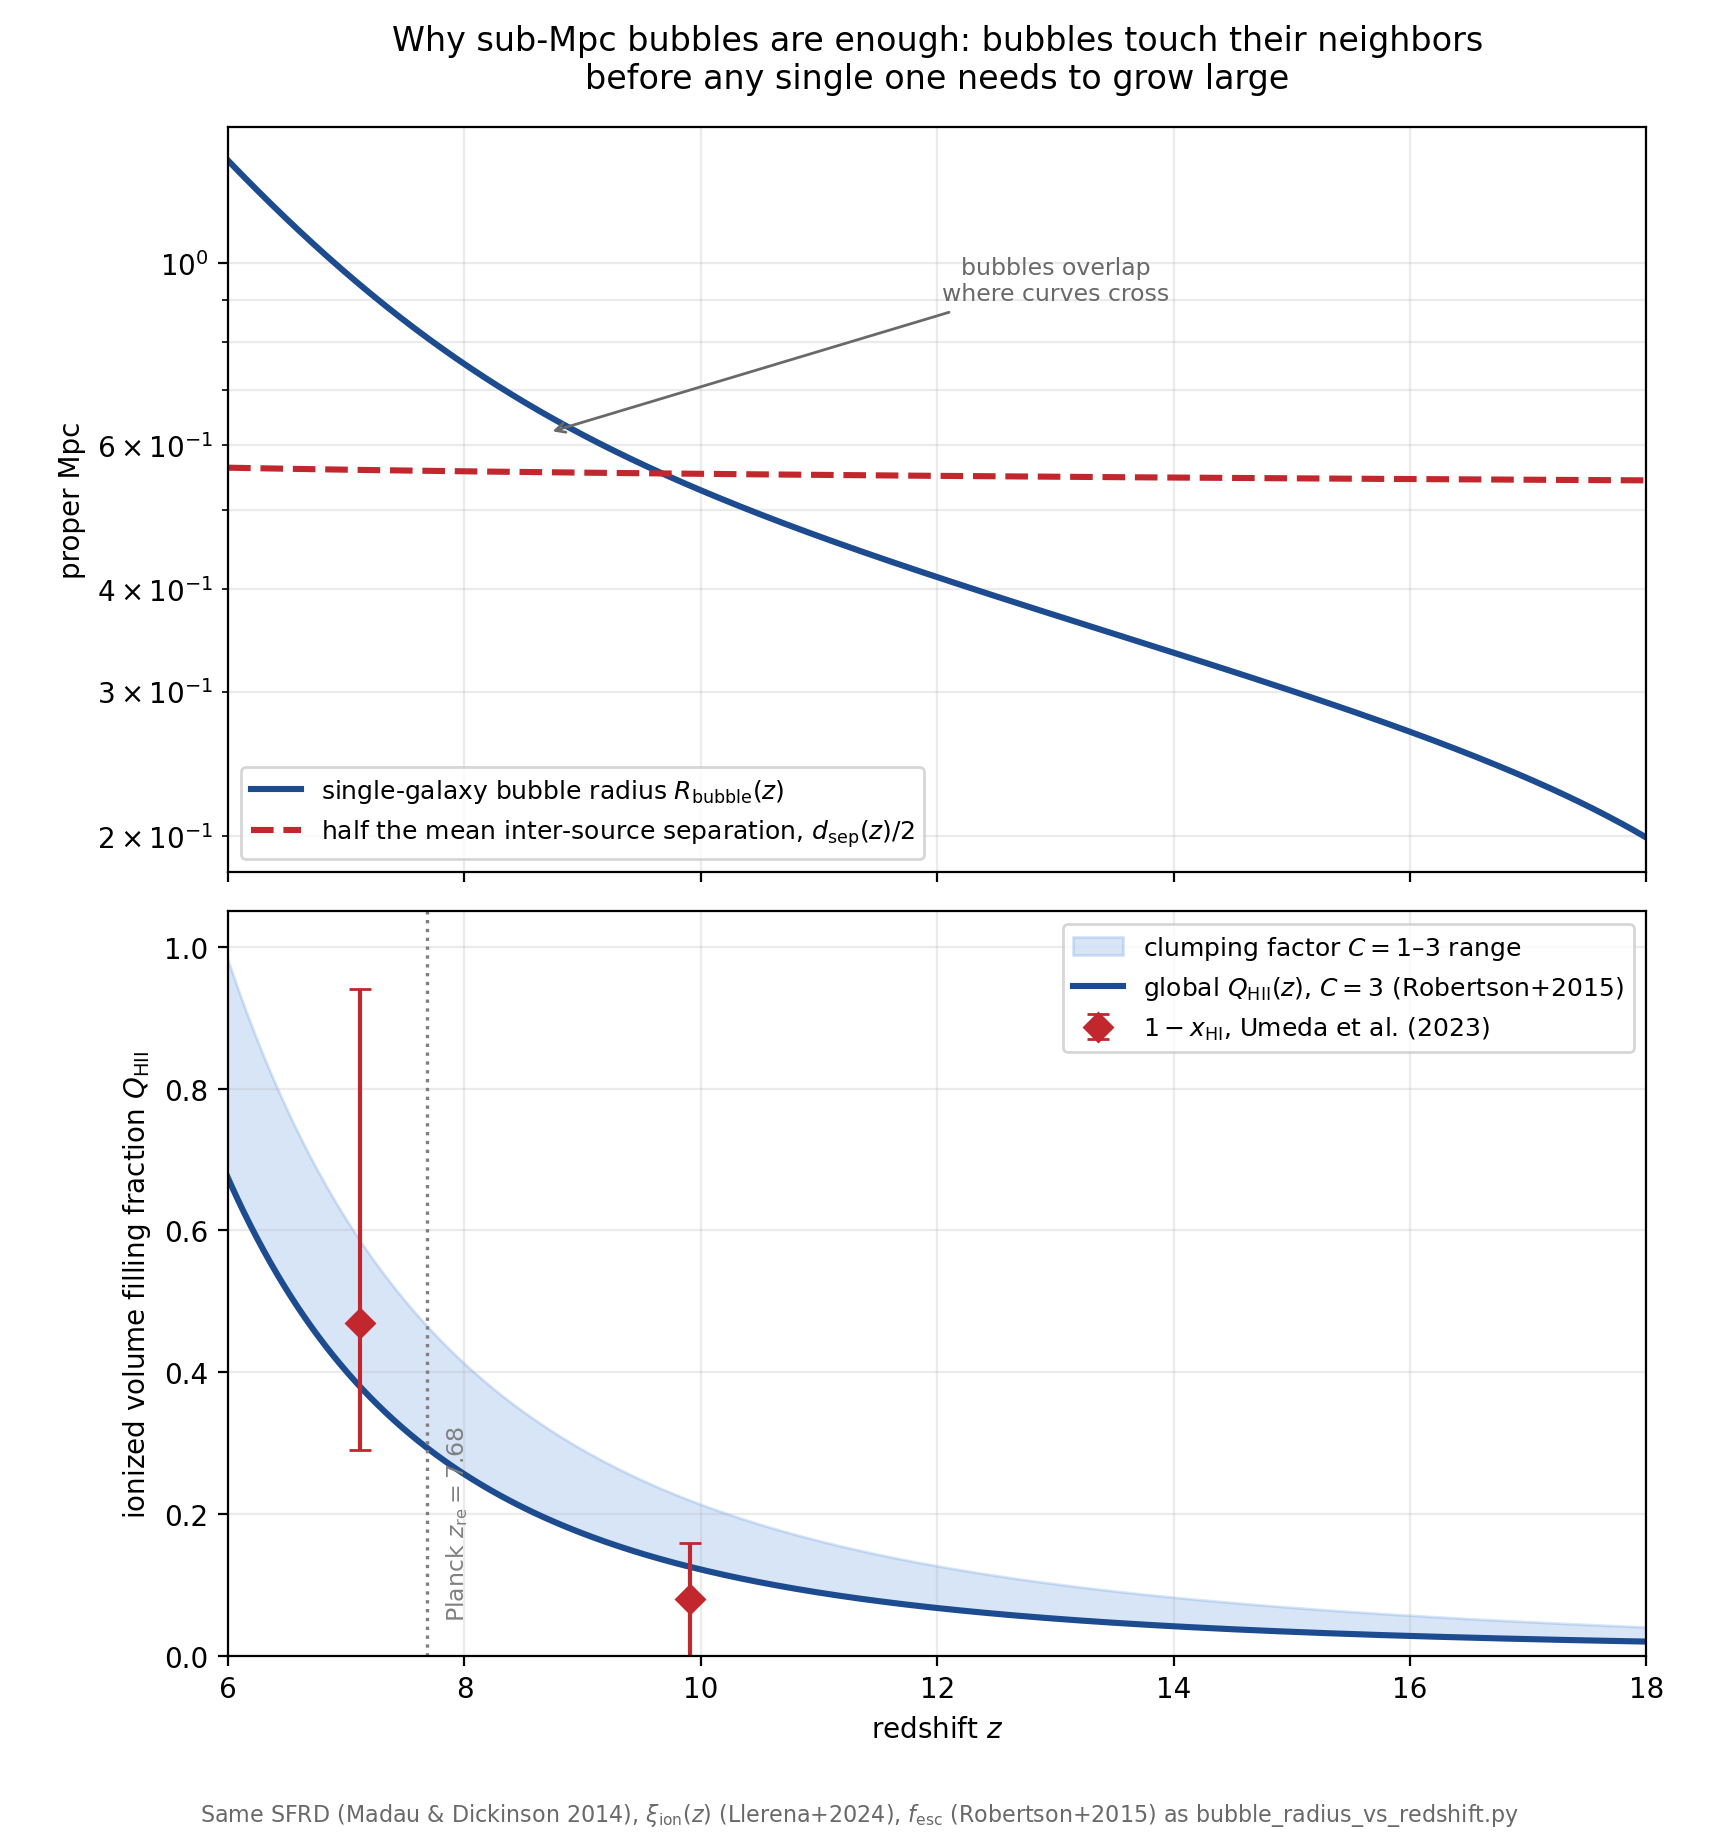
\includegraphics[width=0.85\textwidth]{reionization_completion.png}
\caption{\emph{Top:} single-galaxy bubble radius $R_{\rm bubble}(z)$ (same fiducial galaxy as
\texttt{bubble\_radius\_vs\_redshift.py}) compared with half the mean inter-source separation
$d_{\rm sep}(z)/2$ implied by the same cosmic SFRD \citep{MadauDickinson2014}; the curves cross near
$z\approx9.5$, marking where neighboring bubbles start to overlap. \emph{Bottom:} the resulting global
ionized volume filling fraction $Q_{\rm HII}(z)$ from eq.~(\ref{eq:QHII}) (shaded: clumping factor
$C=1$--$3$), compared with the directly measured $1-x_{\rm HI}$ of \citet{Umeda2023} and the Planck
2018 instantaneous-reionization redshift \citep{Planck2018VI}. Produced by
\texttt{reionization\_completion.py}.}
\label{fig:reionization}
\end{figure}

%=====================================================================
\bibliography{references}

\end{document}
